\documentclass[utf8]{ctexart}

\usepackage[a4paper,left=1.25in,right=1.25in,top=1in,bottom=1in]{geometry}
\usepackage{listings}
\usepackage{graphicx}
\usepackage{caption}
\usepackage{subfigure}
\usepackage{booktabs}
\usepackage{amsmath}
\usepackage{amsthm}
\usepackage{amsfonts}
\usepackage{float}
\usepackage{indentfirst}
\usepackage{tikz}
\usetikzlibrary{shapes,arrows}
\usetikzlibrary{shapes.geometric, arrows}
\usepackage{algorithm}
\usepackage{algorithmic}
\usepackage{newclude}
\usepackage[perpage]{footmisc}

\graphicspath{ {images/} }
\raggedbottom	% 令页面在垂直方向向顶部对齐
\renewcommand\qedsymbol{QED}
\newcommand{\sign}[1]{\mathrm{sgn}(#1)}
\everymath{\displaystyle}   % 行内公式采用行间公式格式排列
\pagestyle{plain}

\title{《计算机辅助几何设计》第五次作业}
\author{姓名:殷文良\qquad 学号:12435063}
\date{\today}

\begin{document}
\maketitle
\ctexset { section = { format={\Large \bfseries } } }

\section*{思考题 1}

\section*{思考题 2}

\section*{思考题 3}
\subsection*{1.}
\begin{itemize}
    \item 次数$p=3$,节点向量$u = [0, 0, 0, 0, 1/2, 1, 1, 1, 1]$,控制顶点
    $p_0=(-1,0)', p_1=(0,1)', p_2=(2,2)', p_3=(1,0)', p_4=(0,-1)'$。
    \begin{figure}[H]
        \centering
        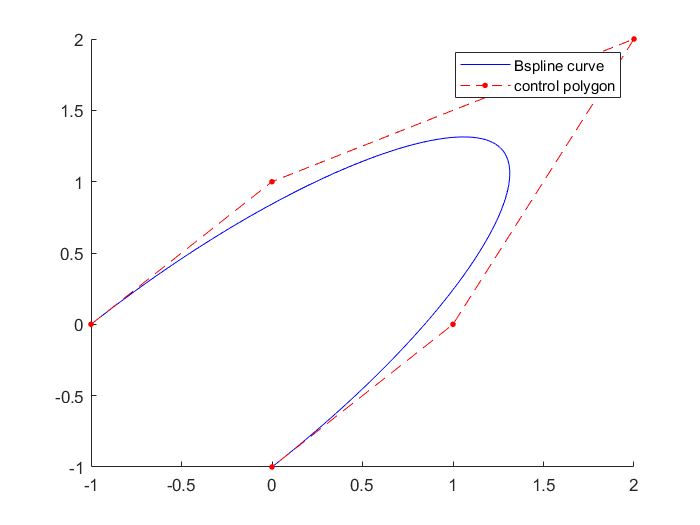
\includegraphics[width=0.8\textwidth]{bspline_2d_1.png}
        \label{fig: bspline_2d_1}
        \caption{2维B-spline曲线}
    \end{figure}
    \begin{figure}[H]
        \centering
        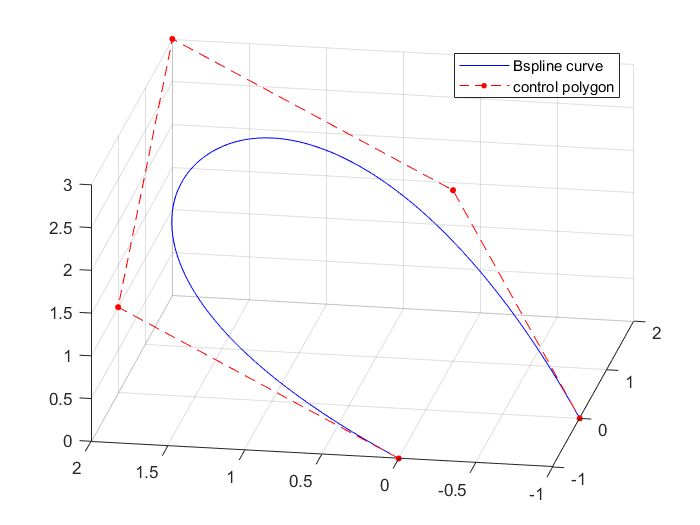
\includegraphics[width=0.8\textwidth]{bspline_3d_1.png}
        \label{fig: bspline_3d_1}
        \caption{3维B-spline曲线}
    \end{figure}
    \item 次数$p=2$,节点向量$u = [0, 0, 0, 1/3, 2/3, 1, 1, 1]$,控制顶点
    $p_0=(-1,0)', p_1=(0,1)', p_2=(2,2)', p_3=(1,0)', p_4=(0,-1)'$。
    \begin{figure}[H]
        \centering
        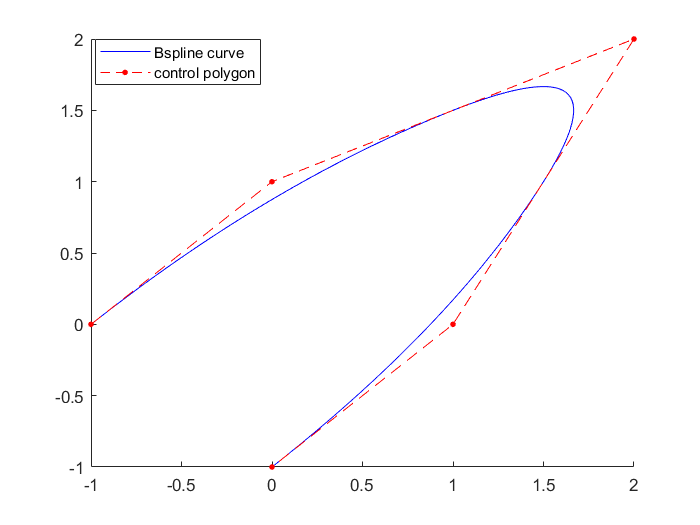
\includegraphics[width=0.8\textwidth]{bspline_2d_2.png}
        \label{fig: bspline_2d_2}
        \caption{2维B-spline曲线}
    \end{figure}
    \begin{figure}[H]
        \centering
        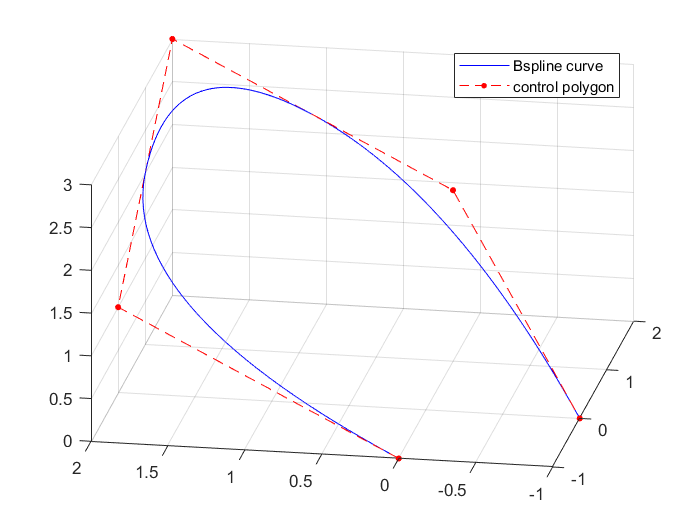
\includegraphics[width=0.8\textwidth]{bspline_3d_2.png}
        \label{fig: bspline_3d_2}
        \caption{3维B-spline曲线}
    \end{figure}
\end{itemize}


\end{document}
